\documentclass[11pt]{article}
\usepackage[margin=1in]{geometry}
\usepackage{graphicx}
\usepackage{booktabs}
\usepackage{amsmath}
\graphicspath{{./}{figures/}}
% AUTO-GENERATED by run_chunked.py --emit — DO NOT EDIT BY HAND.
\newcommand{\BBCNACdeRankedIspyTwoStagepassApoptosisOn}{39}
\newcommand{\BBCNACdeRankedIspyTwoStagepassProliferationOff}{60}
\newcommand{\BBCNACdeRankedIspyTwoStagepassResistanceOff}{13}
\newcommand{\BBCNACdeRankedIspyTwoStagepassTerminal}{4}
\newcommand{\BBCNACdeRankedMetabricStagepassApoptosisOn}{33}
\newcommand{\BBCNACdeRankedMetabricStagepassProliferationOff}{61}
\newcommand{\BBCNACdeRankedMetabricStagepassResistanceOff}{7}
\newcommand{\BBCNACdeRankedMetabricStagepassTerminal}{1}
\newcommand{\BBCNACdeRankedTcgaStagepassApoptosisOn}{31}
\newcommand{\BBCNACdeRankedTcgaStagepassProliferationOff}{65}
\newcommand{\BBCNACdeRankedTcgaStagepassResistanceOff}{14}
\newcommand{\BBCNACdeRankedTcgaStagepassTerminal}{4}
\newcommand{\BBCNACdeStabilizeIspyTwoStagepassApoptosisOn}{35}
\newcommand{\BBCNACdeStabilizeIspyTwoStagepassProliferationOff}{43}
\newcommand{\BBCNACdeStabilizeIspyTwoStagepassResistanceOff}{8}
\newcommand{\BBCNACdeStabilizeIspyTwoStagepassTerminal}{3}
\newcommand{\BBCNACdeStabilizeMetabricStagepassApoptosisOn}{29}
\newcommand{\BBCNACdeStabilizeMetabricStagepassProliferationOff}{40}
\newcommand{\BBCNACdeStabilizeMetabricStagepassResistanceOff}{4}
\newcommand{\BBCNACdeStabilizeMetabricStagepassTerminal}{1}
\newcommand{\BBCNACdeStabilizeTcgaStagepassApoptosisOn}{27}
\newcommand{\BBCNACdeStabilizeTcgaStagepassProliferationOff}{39}
\newcommand{\BBCNACdeStabilizeTcgaStagepassResistanceOff}{8}
\newcommand{\BBCNACdeStabilizeTcgaStagepassTerminal}{3}
\newcommand{\BBCNAStaticRankedIspyTwoIsoApoptosisOn}{81}
\newcommand{\BBCNAStaticRankedIspyTwoIsoProliferationOff}{94}
\newcommand{\BBCNAStaticRankedIspyTwoIsoResistanceOff}{8}
\newcommand{\BBCNAStaticRankedIspyTwoN}{988}
\newcommand{\BBCNAStaticRankedIspyTwoSeqAllThree}{3}
\newcommand{\BBCNAStaticRankedIspyTwoSeqApoptosisOn}{9}
\newcommand{\BBCNAStaticRankedIspyTwoSeqProliferationOff}{4}
\newcommand{\BBCNAStaticRankedIspyTwoSeqResistanceOff}{8}
\newcommand{\BBCNAStaticRankedMetabricIsoApoptosisOn}{85}
\newcommand{\BBCNAStaticRankedMetabricIsoProliferationOff}{95}
\newcommand{\BBCNAStaticRankedMetabricIsoResistanceOff}{4}
\newcommand{\BBCNAStaticRankedMetabricN}{1980}
\newcommand{\BBCNAStaticRankedMetabricSeqAllThree}{2}
\newcommand{\BBCNAStaticRankedMetabricSeqApoptosisOn}{5}
\newcommand{\BBCNAStaticRankedMetabricSeqProliferationOff}{2}
\newcommand{\BBCNAStaticRankedMetabricSeqResistanceOff}{4}
\newcommand{\BBCNAStaticRankedTcgaIsoApoptosisOn}{86}
\newcommand{\BBCNAStaticRankedTcgaIsoProliferationOff}{94}
\newcommand{\BBCNAStaticRankedTcgaIsoResistanceOff}{8}
\newcommand{\BBCNAStaticRankedTcgaN}{1082}
\newcommand{\BBCNAStaticRankedTcgaSeqAllThree}{3}
\newcommand{\BBCNAStaticRankedTcgaSeqApoptosisOn}{9}
\newcommand{\BBCNAStaticRankedTcgaSeqProliferationOff}{3}
\newcommand{\BBCNAStaticRankedTcgaSeqResistanceOff}{8}
\newcommand{\BBCNAStaticStabilizeIspyTwoIsoApoptosisOn}{87}
\newcommand{\BBCNAStaticStabilizeIspyTwoIsoProliferationOff}{91}
\newcommand{\BBCNAStaticStabilizeIspyTwoIsoResistanceOff}{5}
\newcommand{\BBCNAStaticStabilizeIspyTwoN}{988}
\newcommand{\BBCNAStaticStabilizeIspyTwoSeqAllThree}{2}
\newcommand{\BBCNAStaticStabilizeIspyTwoSeqApoptosisOn}{12}
\newcommand{\BBCNAStaticStabilizeIspyTwoSeqProliferationOff}{2}
\newcommand{\BBCNAStaticStabilizeIspyTwoSeqResistanceOff}{5}
\newcommand{\BBCNAStaticStabilizeMetabricIsoApoptosisOn}{89}
\newcommand{\BBCNAStaticStabilizeMetabricIsoProliferationOff}{91}
\newcommand{\BBCNAStaticStabilizeMetabricIsoResistanceOff}{3}
\newcommand{\BBCNAStaticStabilizeMetabricN}{1980}
\newcommand{\BBCNAStaticStabilizeMetabricSeqAllThree}{1}
\newcommand{\BBCNAStaticStabilizeMetabricSeqApoptosisOn}{6}
\newcommand{\BBCNAStaticStabilizeMetabricSeqProliferationOff}{1}
\newcommand{\BBCNAStaticStabilizeMetabricSeqResistanceOff}{3}
\newcommand{\BBCNAStaticStabilizeTcgaIsoApoptosisOn}{91}
\newcommand{\BBCNAStaticStabilizeTcgaIsoProliferationOff}{85}
\newcommand{\BBCNAStaticStabilizeTcgaIsoResistanceOff}{5}
\newcommand{\BBCNAStaticStabilizeTcgaN}{1082}
\newcommand{\BBCNAStaticStabilizeTcgaSeqAllThree}{2}
\newcommand{\BBCNAStaticStabilizeTcgaSeqApoptosisOn}{11}
\newcommand{\BBCNAStaticStabilizeTcgaSeqProliferationOff}{2}
\newcommand{\BBCNAStaticStabilizeTcgaSeqResistanceOff}{5}
\newcommand{\BBCNBKernelRankedIspyTwoFlipPct}{46}
\newcommand{\BBCNBKernelRankedIspyTwoKerDesigned}{430}
\newcommand{\BBCNBKernelRankedIspyTwoKerSuccess}{198}
\newcommand{\BBCNBKernelRankedIspyTwoTopNode}{PIK3CA}
\newcommand{\BBCNBKernelRankedMetabricFlipPct}{42}
\newcommand{\BBCNBKernelRankedMetabricKerDesigned}{890}
\newcommand{\BBCNBKernelRankedMetabricKerSuccess}{373}
\newcommand{\BBCNBKernelRankedMetabricTopNode}{PIK3CA}
\newcommand{\BBCNBKernelRankedTcgaFlipPct}{47}
\newcommand{\BBCNBKernelRankedTcgaKerDesigned}{428}
\newcommand{\BBCNBKernelRankedTcgaKerSuccess}{202}
\newcommand{\BBCNBKernelRankedTcgaTopNode}{PIK3CA}
\newcommand{\BBCNBKernelStabilizeIspyTwoFlipPct}{46}
\newcommand{\BBCNBKernelStabilizeIspyTwoKerDesigned}{430}
\newcommand{\BBCNBKernelStabilizeIspyTwoKerSuccess}{198}
\newcommand{\BBCNBKernelStabilizeIspyTwoTopNode}{PIK3CA}
\newcommand{\BBCNBKernelStabilizeMetabricFlipPct}{42}
\newcommand{\BBCNBKernelStabilizeMetabricKerDesigned}{890}
\newcommand{\BBCNBKernelStabilizeMetabricKerSuccess}{373}
\newcommand{\BBCNBKernelStabilizeMetabricTopNode}{PIK3CA}
\newcommand{\BBCNBKernelStabilizeTcgaFlipPct}{47}
\newcommand{\BBCNBKernelStabilizeTcgaKerDesigned}{428}
\newcommand{\BBCNBKernelStabilizeTcgaKerSuccess}{202}
\newcommand{\BBCNBKernelStabilizeTcgaTopNode}{PIK3CA}
\newcommand{\BBCNBRoutingSwitchIspyTwoApopPct}{51}
\newcommand{\BBCNBRoutingSwitchIspyTwoMixedPct}{23}
\newcommand{\BBCNBRoutingSwitchIspyTwoN}{988}
\newcommand{\BBCNBRoutingSwitchIspyTwoResistApopZ}{0.08}
\newcommand{\BBCNBRoutingSwitchIspyTwoResistSurvZ}{0.32}
\newcommand{\BBCNBRoutingSwitchIspyTwoSurvPct}{25}
\newcommand{\BBCNBRoutingSwitchIspyTwoSurvUncoupledPct}{89}
\newcommand{\BBCNBRoutingSwitchIspyTwoUPct}{26}
\newcommand{\BBCNBRoutingSwitchMetabricApopPct}{48}
\newcommand{\BBCNBRoutingSwitchMetabricMixedPct}{22}
\newcommand{\BBCNBRoutingSwitchMetabricN}{1980}
\newcommand{\BBCNBRoutingSwitchMetabricResistApopZ}{0.11}
\newcommand{\BBCNBRoutingSwitchMetabricResistSurvZ}{0.2}
\newcommand{\BBCNBRoutingSwitchMetabricSurvPct}{29}
\newcommand{\BBCNBRoutingSwitchMetabricSurvUncoupledPct}{90}
\newcommand{\BBCNBRoutingSwitchMetabricUPct}{29}
\newcommand{\BBCNBRoutingSwitchTcgaApopPct}{50}
\newcommand{\BBCNBRoutingSwitchTcgaMixedPct}{14}
\newcommand{\BBCNBRoutingSwitchTcgaN}{1082}
\newcommand{\BBCNBRoutingSwitchTcgaResistApopZ}{0.32}
\newcommand{\BBCNBRoutingSwitchTcgaResistSurvZ}{0.8}
\newcommand{\BBCNBRoutingSwitchTcgaSurvPct}{36}
\newcommand{\BBCNBRoutingSwitchTcgaSurvUncoupledPct}{95}
\newcommand{\BBCNBRoutingSwitchTcgaUPct}{37}

% AUTO-GENERATED by generate_numbers2.py - DO NOT EDIT BY HAND.
% Repaired-network (paper 3) numbers. Generated 2026-06-18.
\newcommand{\BBCNRepairResistUncouplingMatch}{4049}
\newcommand{\BBCNRepairResistUncouplingTotal}{4050}
\newcommand{\BBCNRepairResistUncouplingPct}{99.98}
\newcommand{\BBCNRepairTcgaUpct}{65}
\newcommand{\BBCNRepairTcgaDrugFlipPct}{35}
\newcommand{\BBCNRepairTcgaGenotoxicPct}{4}
\newcommand{\BBCNRepairTcgaResistantPct}{48}
\newcommand{\BBCNRepairTcgaKernelFoundPct}{100}
\newcommand{\BBCNRepairTcgaSwitchDurablePct}{80}
\newcommand{\BBCNRepairTcgaFullnetStrictPct}{12}
\newcommand{\BBCNRepairTcgaFullnetCommitPct}{93}
\newcommand{\BBCNRepairTcgaApoptosisPct}{78}
\newcommand{\BBCNRepairTcgaProliferationPct}{86}
\newcommand{\BBCNRepairTcgaJointPct}{13}
\newcommand{\BBCNRepairTcgaDurablePct}{17}
\newcommand{\BBCNRepairMetabricUpct}{64}
\newcommand{\BBCNRepairMetabricDrugFlipPct}{36}
\newcommand{\BBCNRepairMetabricGenotoxicPct}{3}
\newcommand{\BBCNRepairMetabricResistantPct}{49}
\newcommand{\BBCNRepairMetabricKernelFoundPct}{99}
\newcommand{\BBCNRepairMetabricSwitchDurablePct}{81}
\newcommand{\BBCNRepairMetabricFullnetStrictPct}{8}
\newcommand{\BBCNRepairMetabricFullnetCommitPct}{92}
\newcommand{\BBCNRepairMetabricApoptosisPct}{76}
\newcommand{\BBCNRepairMetabricProliferationPct}{87}
\newcommand{\BBCNRepairMetabricJointPct}{7}
\newcommand{\BBCNRepairMetabricDurablePct}{15}
\newcommand{\BBCNRepairIspyTwoUpct}{67}
\newcommand{\BBCNRepairIspyTwoDrugFlipPct}{33}
\newcommand{\BBCNRepairIspyTwoGenotoxicPct}{3}
\newcommand{\BBCNRepairIspyTwoResistantPct}{52}
\newcommand{\BBCNRepairIspyTwoKernelFoundPct}{99}
\newcommand{\BBCNRepairIspyTwoSwitchDurablePct}{84}
\newcommand{\BBCNRepairIspyTwoFullnetStrictPct}{14}
\newcommand{\BBCNRepairIspyTwoFullnetCommitPct}{95}
\newcommand{\BBCNRepairIspyTwoApoptosisPct}{72}
\newcommand{\BBCNRepairIspyTwoProliferationPct}{84}
\newcommand{\BBCNRepairIspyTwoJointPct}{14}
\newcommand{\BBCNRepairIspyTwoDurablePct}{16}
\newcommand{\BBCNRepairUpctRange}{64--67}
\newcommand{\BBCNRepairDrugFlipRange}{33--36}
\newcommand{\BBCNRepairGenotoxicRange}{3--4}
\newcommand{\BBCNRepairResistantRange}{48--52}
\newcommand{\BBCNRepairKernelFoundRange}{99--100}
\newcommand{\BBCNRepairSwitchDurableRange}{80--84}
\newcommand{\BBCNRepairStrictRange}{8--14}
\newcommand{\BBCNRepairCommitRange}{92--95}
\newcommand{\BBCNRepairApoptosisRange}{72--78}
\newcommand{\BBCNRepairProliferationRange}{84--87}
\newcommand{\BBCNRepairJointRange}{7--14}
\newcommand{\BBCNRepairDurableRange}{15--17}


\title{Supplementary Information\\
The Boolean Breast-Cancer Network (BBCN), Paper 3 v2}
\date{}
\begin{document}
\maketitle

\section*{S1. The two kernel methods and the two controllers, compared}

This supplement gives the full comparison summarised in Section~3.8 of the main
text. Both kernel designs, the ranked reachability heuristic and the algebraic
global-stabilisation test (Methods, Tier~1), were run on both the static
controller (which fixes the per-phenotype pathway set) and the dynamic
whole-network controller (which selects pathways by failure classification), on
all three cohorts at full $N$, on the bare, un-repaired 135-node network under
synchronous updating. Table~\ref{tab:compareS} reports the per-phenotype results;
routing in Setup~B is unaffected by the kernel method, since kernels are designed
only after a patient is routed. In the figures the algebraic method is labelled
\emph{stabilize} and the heuristic \emph{ranked}; these are two names for the same
kernel-selection step.

Three readings follow. First, the ranked method reproduces the earlier BBCN118
kernels exactly, so the heuristic results are preserved rather than discarded.
Second, on the static controller the two methods are close (apoptosis differs by
at most a few points), because for the per-pathway targets used here the patient's
own state already lies in the stabilising basin. Third, on the dynamic controller
the algebraic method certifies fewer passes than the heuristic, the gap being
largest on proliferation (TCGA \BBCNACdeRankedTcgaStagepassProliferationOff\%
ranked versus \BBCNACdeStabilizeTcgaStagepassProliferationOff\% algebraic), because
it demands that the clamp drive \emph{every} pathway state to target, not only the
patient's starting state. The algebraic figure is the conservative, provable one;
the difference between the two columns is exactly the set of patients the heuristic
counts from a favourable initial state that are not globally stabilisable. In
Setup~B the two methods give identical flip rates in every cohort (TCGA
\BBCNBKernelRankedTcgaFlipPct\% vs \BBCNBKernelStabilizeTcgaFlipPct\%, METABRIC
\BBCNBKernelRankedMetabricFlipPct\% vs \BBCNBKernelStabilizeMetabricFlipPct\%,
I-SPY2 \BBCNBKernelRankedIspyTwoFlipPct\% vs \BBCNBKernelStabilizeIspyTwoFlipPct\%),
with PIK3CA the leading actuator throughout: on the small bistable boxes the
algebraic test confirms the heuristic kernel rather than contradicting it.

\begin{table}[h]
\centering
\caption{\textbf{Table S1.} Kernel-method and controller comparison (\% reaching
target), full cohorts, bare 135-node network. Static = fixed pathway set;
Dynamic = whole-network failure-classification selection. Each cell pair is
ranked\,$\vert$\,algebraic.}
\label{tab:compareS}
\begin{tabular}{llcccc}
\toprule
& & \multicolumn{2}{c}{Static controller} & \multicolumn{2}{c}{Dynamic (whole-network)} \\
\cmidrule(lr){3-4}\cmidrule(lr){5-6}
Cohort & Phenotype & ranked & algebraic & ranked & algebraic \\
\midrule
TCGA     & Apoptosis      & \BBCNAStaticRankedTcgaIsoApoptosisOn & \BBCNAStaticStabilizeTcgaIsoApoptosisOn & \BBCNACdeRankedTcgaStagepassApoptosisOn & \BBCNACdeStabilizeTcgaStagepassApoptosisOn \\
         & Proliferation  & \BBCNAStaticRankedTcgaIsoProliferationOff & \BBCNAStaticStabilizeTcgaIsoProliferationOff & \BBCNACdeRankedTcgaStagepassProliferationOff & \BBCNACdeStabilizeTcgaStagepassProliferationOff \\
METABRIC & Apoptosis      & \BBCNAStaticRankedMetabricIsoApoptosisOn & \BBCNAStaticStabilizeMetabricIsoApoptosisOn & \BBCNACdeRankedMetabricStagepassApoptosisOn & \BBCNACdeStabilizeMetabricStagepassApoptosisOn \\
         & Proliferation  & \BBCNAStaticRankedMetabricIsoProliferationOff & \BBCNAStaticStabilizeMetabricIsoProliferationOff & \BBCNACdeRankedMetabricStagepassProliferationOff & \BBCNACdeStabilizeMetabricStagepassProliferationOff \\
I-SPY2   & Apoptosis      & \BBCNAStaticRankedIspyTwoIsoApoptosisOn & \BBCNAStaticStabilizeIspyTwoIsoApoptosisOn & \BBCNACdeRankedIspyTwoStagepassApoptosisOn & \BBCNACdeStabilizeIspyTwoStagepassApoptosisOn \\
         & Proliferation  & \BBCNAStaticRankedIspyTwoIsoProliferationOff & \BBCNAStaticStabilizeIspyTwoIsoProliferationOff & \BBCNACdeRankedIspyTwoStagepassProliferationOff & \BBCNACdeStabilizeIspyTwoStagepassProliferationOff \\
\bottomrule
\end{tabular}
\end{table}

\begin{figure}[h]
\centering
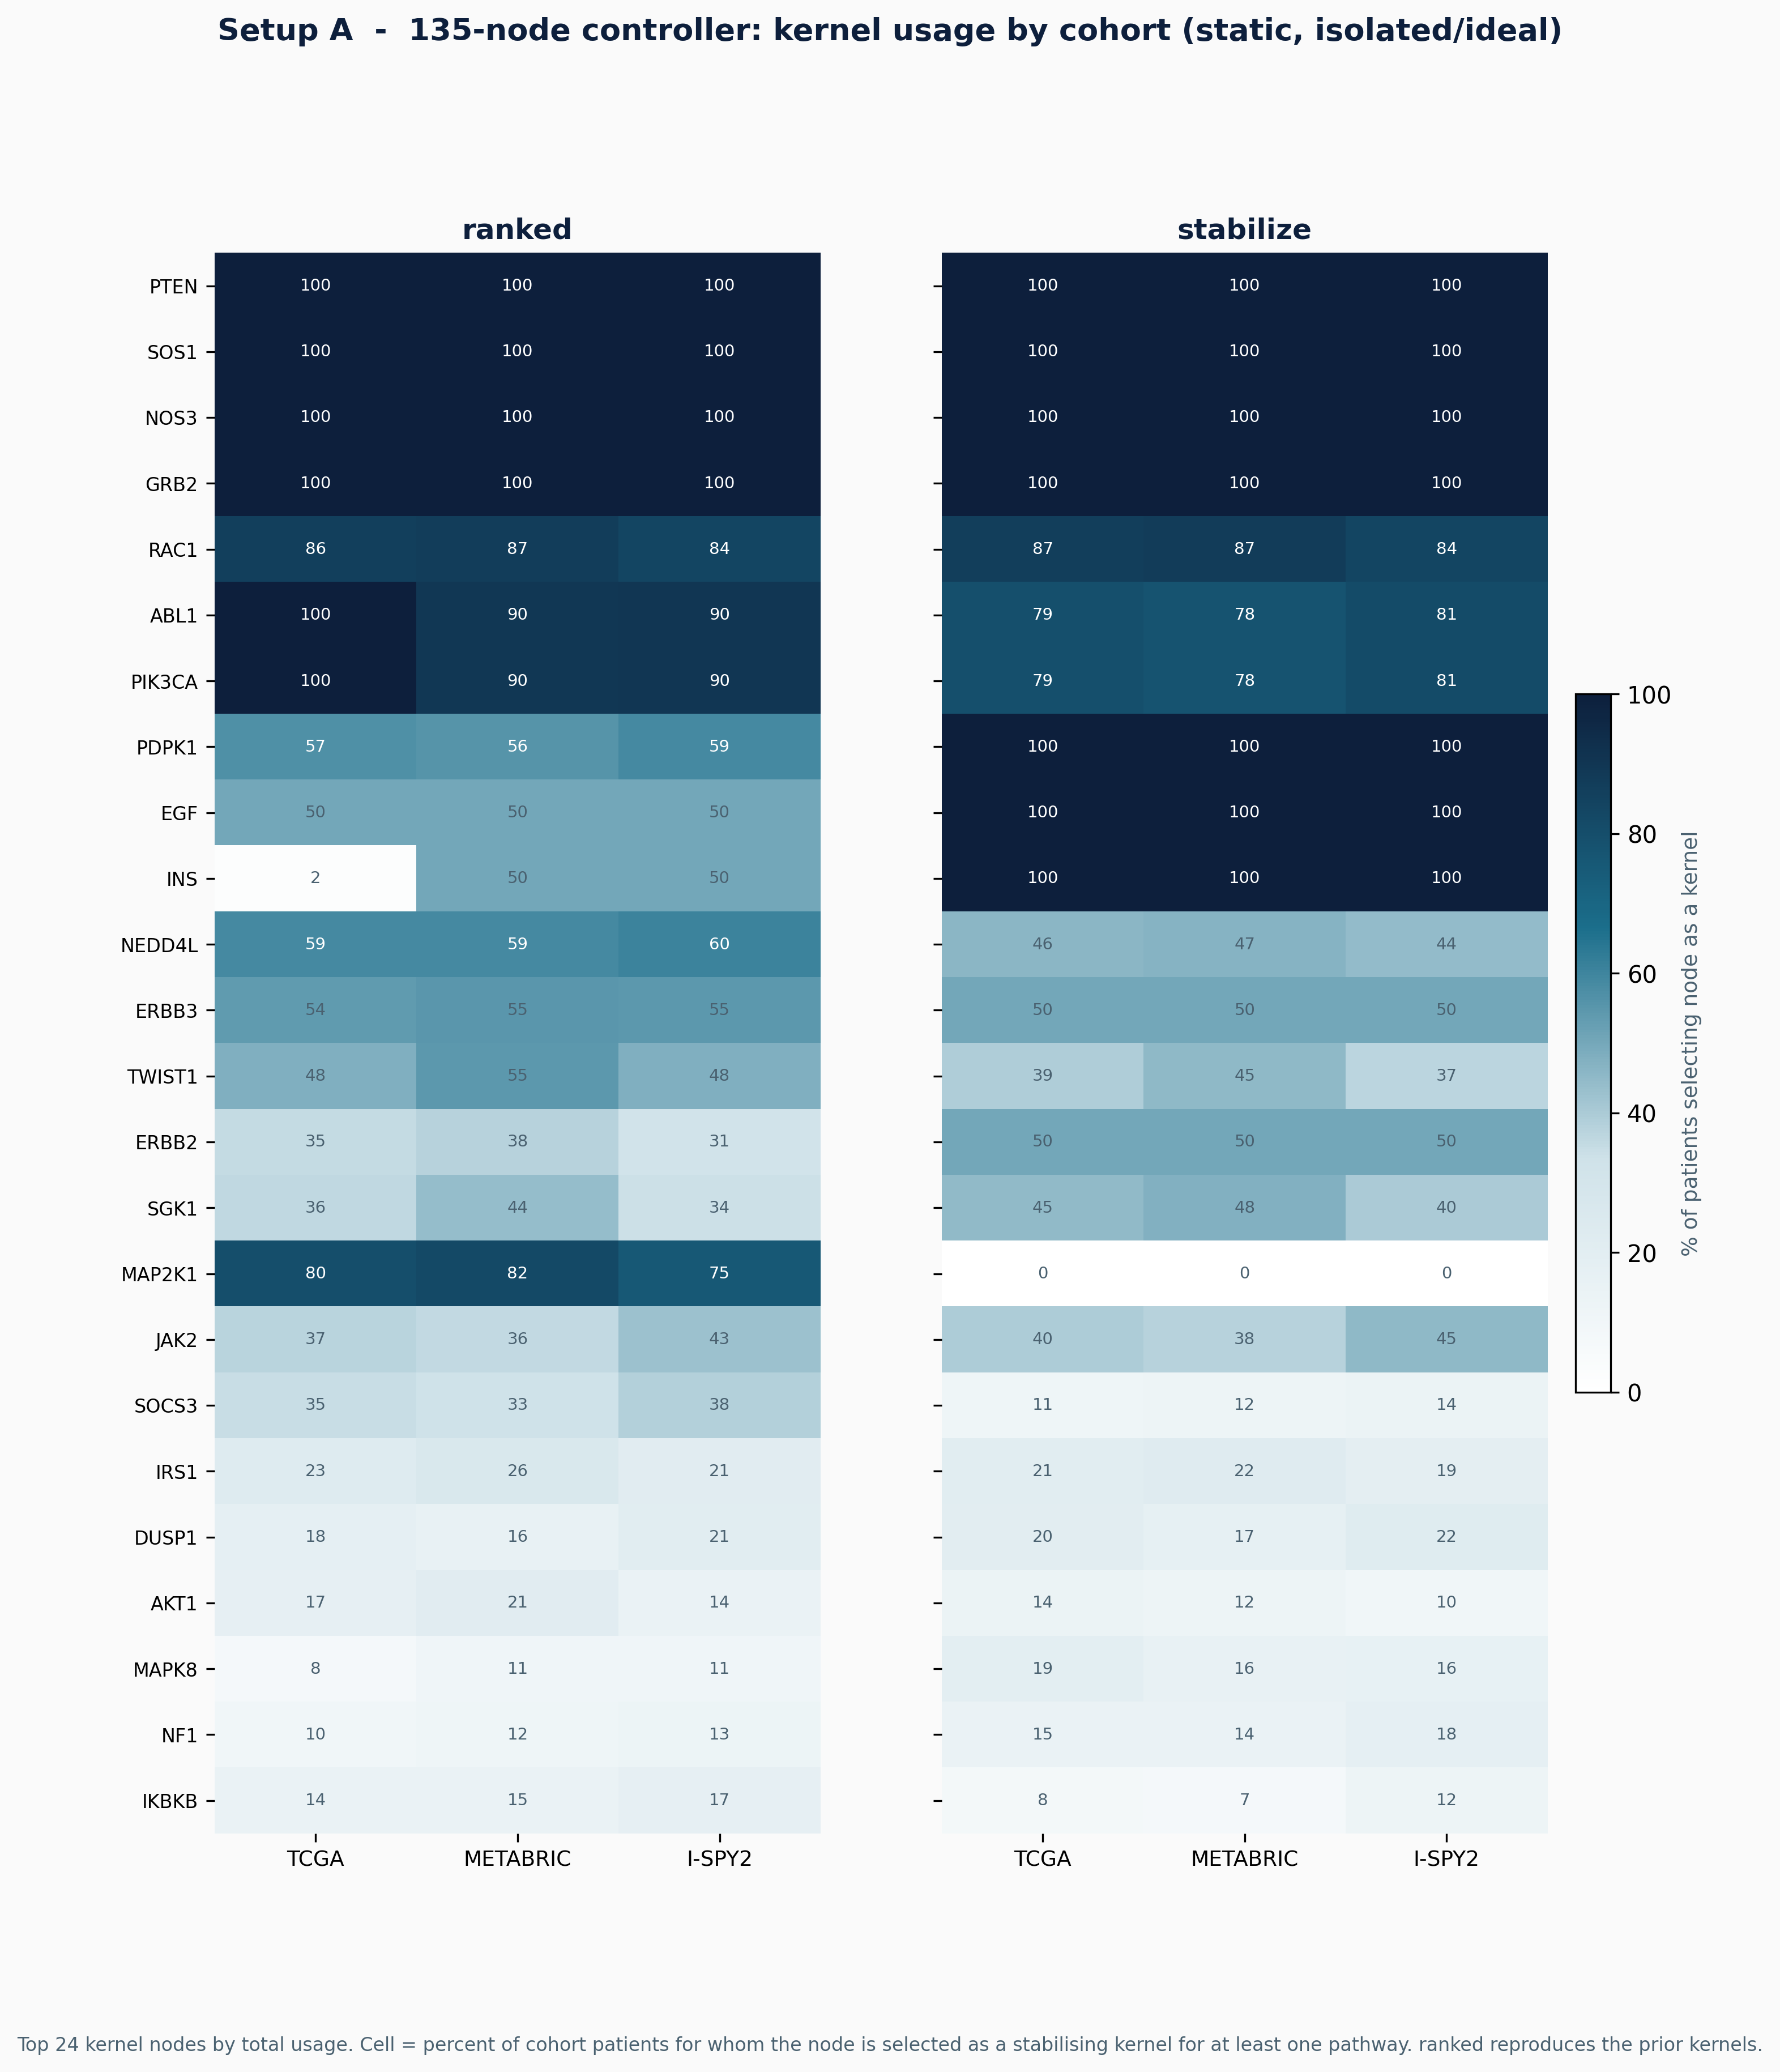
\includegraphics[width=\textwidth]{figures/figA_kernel_usage.png}
\caption{\textbf{Figure S1. Setup~A kernel usage by cohort.} The 24 most-used
kernel nodes under the static, isolated/ideal controller, shown for the ranked
heuristic (left) and the algebraic (stabilize) test (right); each cell is the
percentage of cohort patients for whom the node is selected as a stabilising
kernel for at least one pathway. A small core, PTEN, SOS1, NOS3, and GRB2, is used
for every patient in every cohort. The algebraic test sets MAP2K1 to zero and EGF
and INS to full use, reflecting its stricter global-stabilisation criterion, while
the dominant nodes are unchanged. The usage pattern is stable across TCGA,
METABRIC, and I-SPY2.}
\label{fig:kernelAusageS}
\end{figure}

\end{document}
